\documentclass{beamer}
\usepackage[utf8]{inputenc}
\usepackage[ngerman]{babel}
\usepackage{listings}
\usepackage{color}
\usepackage{xcolor}
\usetheme{Antibes}
\begin{document}
\title{Cross-Compiling für den Raspberry Pi auf Linux}   
\author{Christopher Perrin} 
\date{\today} 

\frame{\titlepage} 

\frame{\frametitle{Inhaltsverzeichnis}\tableofcontents} 

\section{Überblick}
\subsection{Kompilieren}
\frame{\begin{Huge}
\begin{center}
Was heißt Kompilieren?
\end{center}
\end{Huge}}


\frame{
\frametitle{Was heißt Kompilieren?}
Kompilieren bedeutet laut Duden:
\begin{quote}
Von einer höheren Programmiersprache in die Maschinensprache eines bestimmten Computers übersetzen
\end{quote}
Im groben heißt das also ...
}

\begin{frame}[fragile]
\frametitle{... wir übersetzen dies ...}
\begin{lstlisting}[language=c, basicstyle=\tiny, tabsize=4, keywordstyle=\color{blue}, commentstyle=\color{green},stringstyle=\color{red}]
#include <linux/module.h>
#include <linux/kdb.h>

static int kdb_hello_cmd(int argc, const char **argv)
{
	if (argc > 1)
		return KDB_ARGCOUNT;

	if (argc)
		kdb_printf("Hello %s.\n", argv[1]);
	else
		kdb_printf("Hello world!\n");

	return 0;
}


static int __init kdb_hello_cmd_init(void)
{
	kdb_register("hello", kdb_hello_cmd, "[string]",
		     "Say Hello World or Hello [string]", 0);
\end{lstlisting}
...
\end{frame}

\begin{frame}[fragile]
\frametitle{...in dies}
\begin{center}
\begin{verbatim}
0000000 8b1f 0008 1bc2 502c 0300 7dec 600d d554
0000010 f095 bf9b 13fc 8202 2202 040e 2825 9984
0000020 91fc 56a0 9848 2181 d240 884c db58 264d
0000030 0793 9033 c4cc 0999 5d24 6dbf ea44 576a
0000040 122d 4a50 b280 b5ad 1fc1 fe0c d67d d5ad
0000050 5add 6dd7 976b c7f4 55ba 7ebb 65b6 ba50
0000060 686d 66ad b76b cefd ef7d cccd ef7d 7bdd
0000070 7bdf 0193 3bb4 3b81 ef33 73bd 3dce def7
0000080 cf73 f73d 73dc 8bef fa45 7f78 a064 b637
0000090 7974 d3b9 34b7 ee1a f88b 65f9 465c 1cff
00000a0 c70e eaf2 3b6a 3b7c 5797 f03b e4ef dd9f
00000b0 e159 5670 ffc2 ca8a bb1a 59c3 5d53 c35d
\end{verbatim}
\end{center}
\end{frame}
\subsection{Architekturen}
\begin{frame}
\begin{center}
\begin{Huge}
Architekturen\\
\end{Huge}
oder\\
\begin{LARGE}
\glqq Nicht jeder Prozessor ist ARM\grqq
\end{LARGE}
\end{center}
\end{frame}

\begin{frame}
\frametitle{Nicht jeder Prozessor ist ARM}
\begin{itemize}
\item Unterschiedliche Prozessor-Architekturen (Typen von Prozessoren)
\item x86, PowerPC, ARM, ...
\item Unterschiedliche Anwendungsgebiete
\begin{itemize}
\item x86: Meistens sehr leistungsstark, eher teuer. Vorrangig verwendet für Desktop PCs, Notebooks, ...
\item ARM: Meistens sehr günstig, effizient, niedriger Stromverbrauch. Meist verwendet für Smartphones, Tablets, Raspberry Pi
\end{itemize}
\item Architekturen Großteils inkompatibel zueinander
\item Da, z.B. ARM nicht sehr leistungsstark, Cross-Compiling sinnvoll
\end{itemize}
\end{frame}

\begin{frame}
\begin{center}
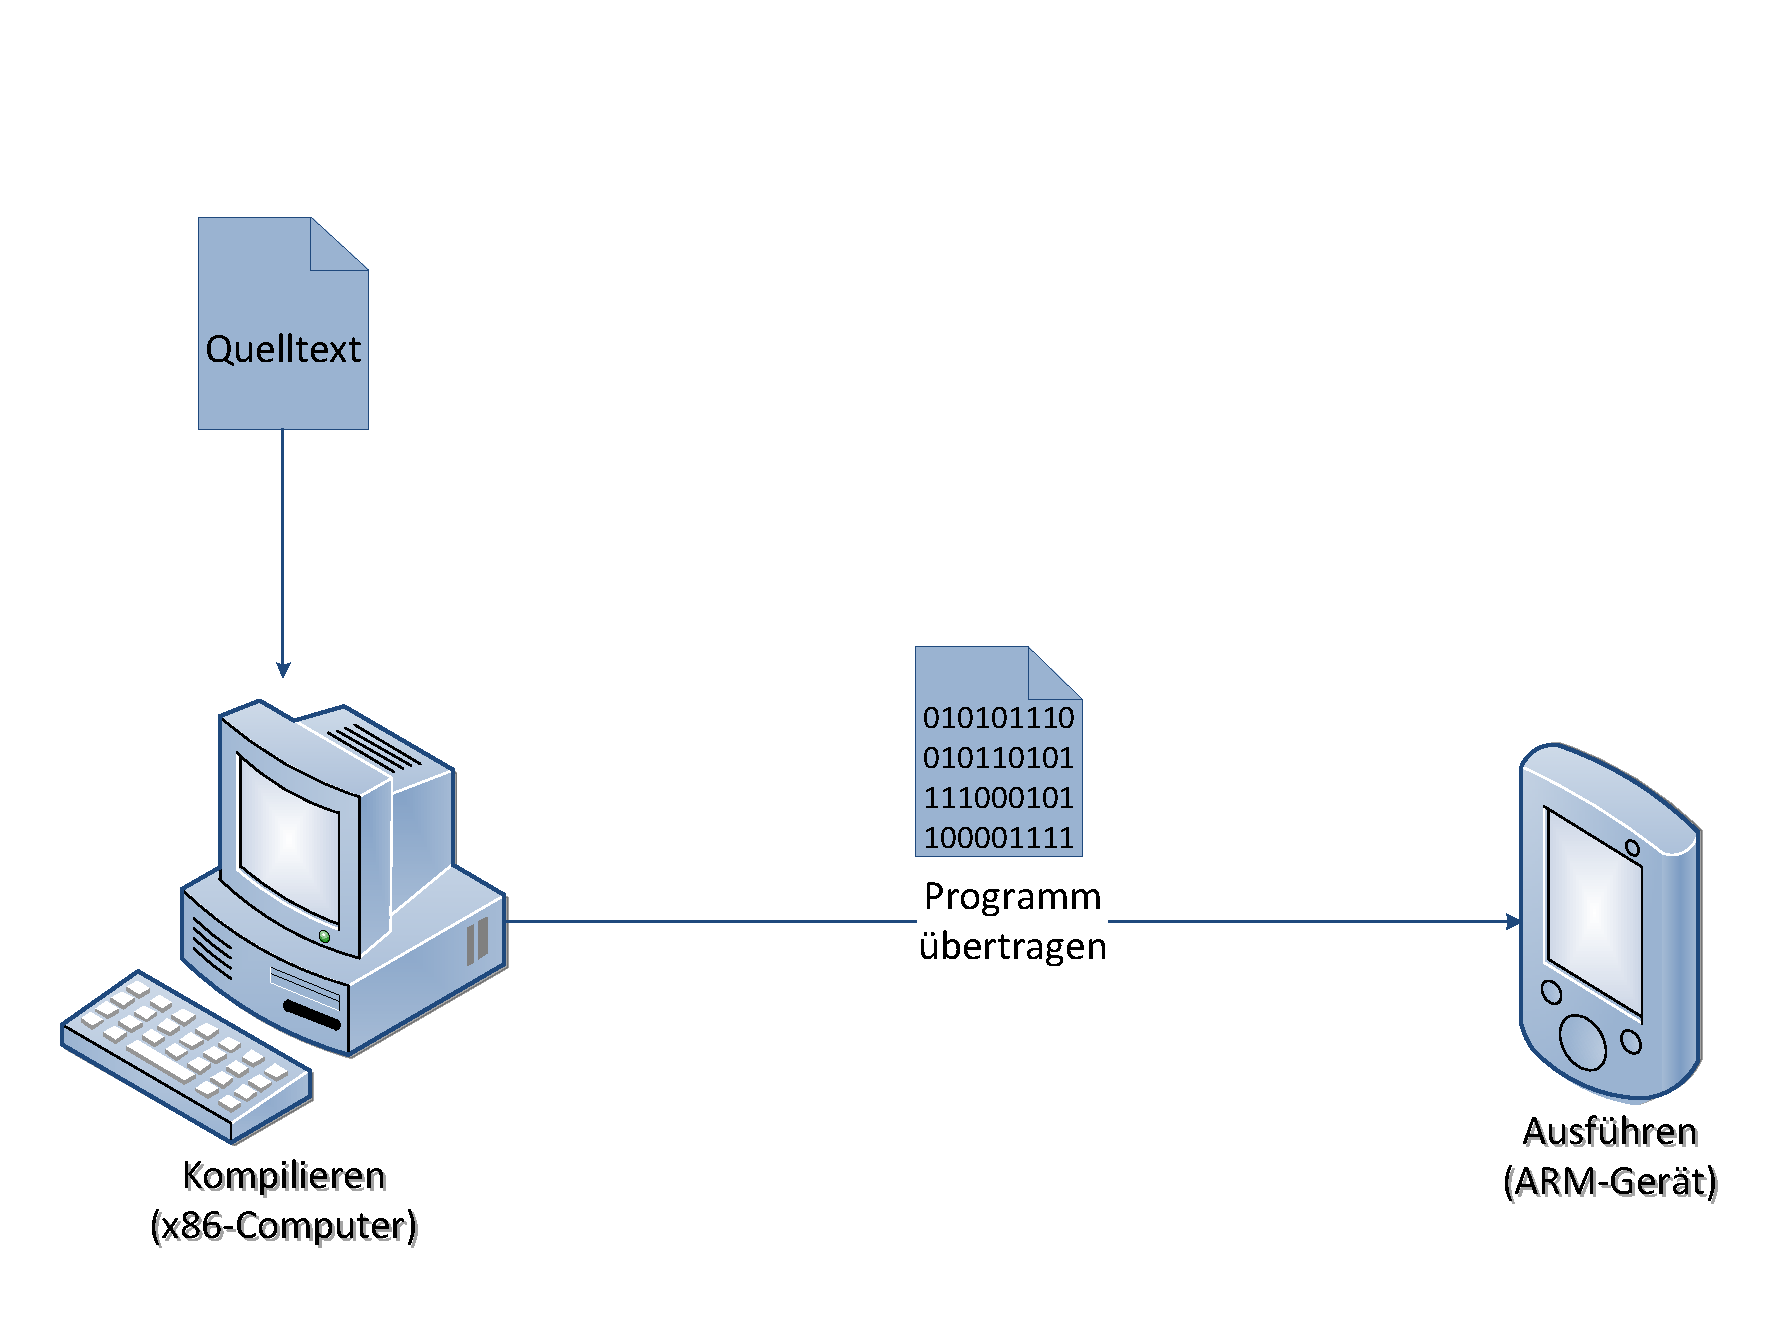
\includegraphics[scale=.3]{image/Cross-compile.pdf} 
\end{center}
\end{frame}

\section{Toolchain}
\begin{frame}
\begin{center}
\begin{Huge}
Toolchain\\
\end{Huge}
oder\\
{\LARGE \glqq Ich bau' mir einen Werkzeuggürtel\grqq}
\end{center}
\end{frame}

\begin{frame}
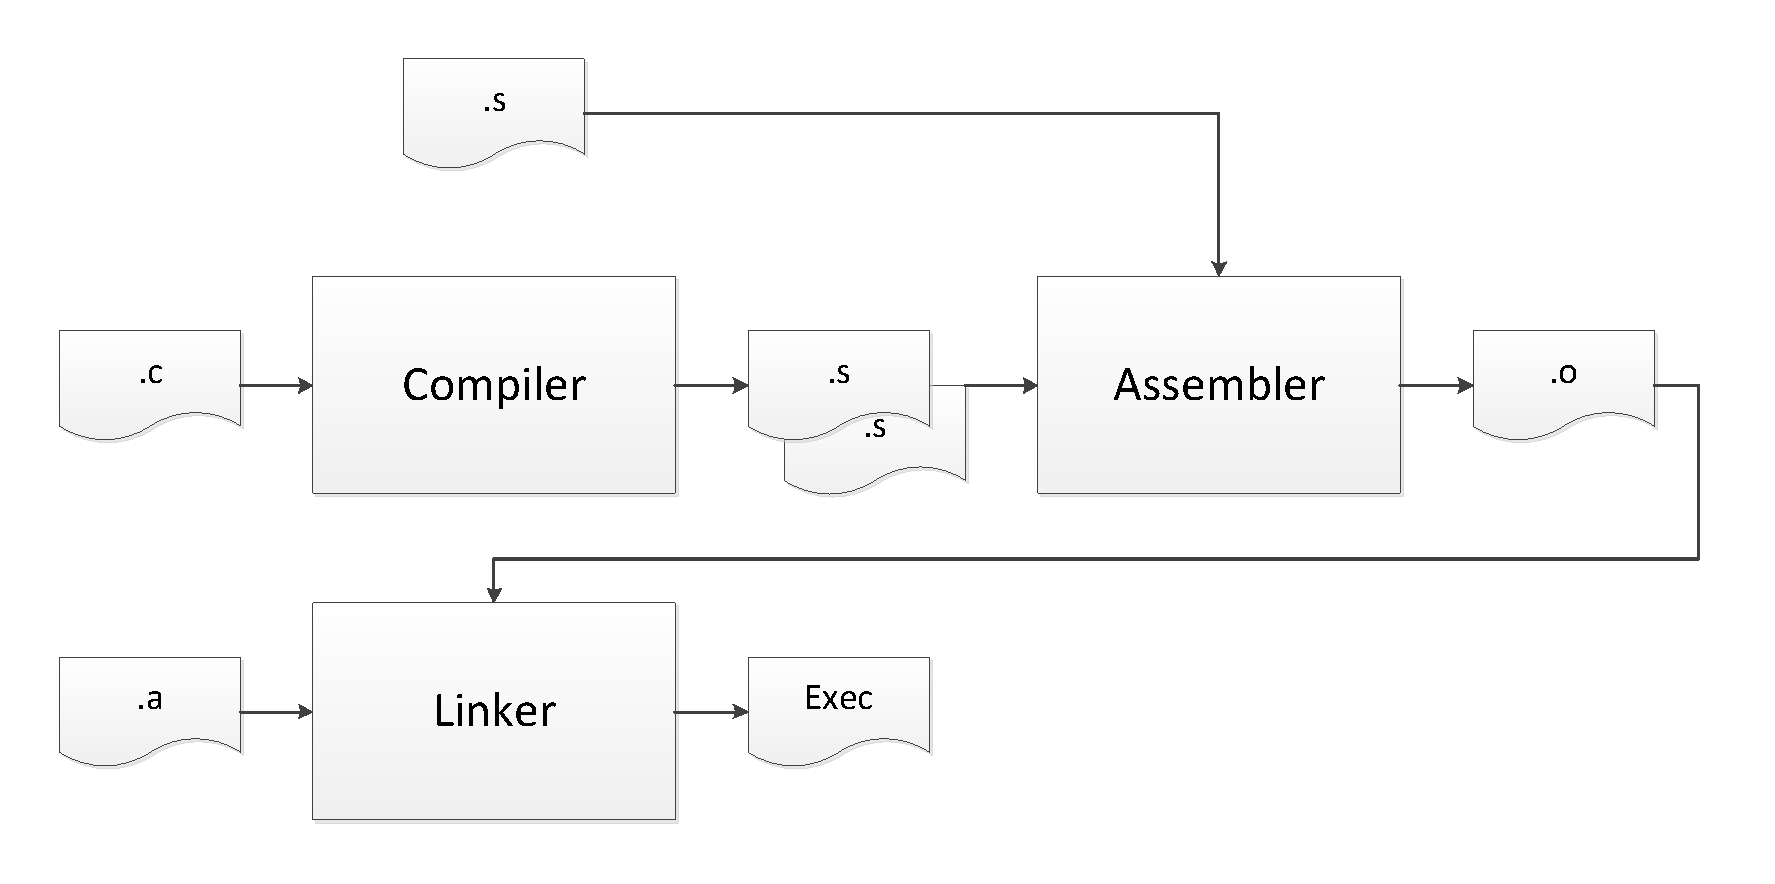
\includegraphics[scale=.35]{image/Toolchain.pdf} 
\end{frame}

\begin{frame}
\frametitle{Ich bau' mir einen Werkzeuggürtel}
\begin{itemize}
\item Zum Kompilieren wird (unter anderem) Compiler benötigt
\item Oft für eigene Architektur schon installiert
\item Für fremde Architektur selber bauen
\item Unser Helferlein: Crosstool-ng
\end{itemize}
\end{frame}

\begin{frame}[fragile]
\frametitle{Crosstool-ng}
\begin{itemize}
\item Die neuste Version von http://crosstool-ng.org/
\item Entpacken und in Ordner wechseln
\item \begin{verbatim}
./configure --prefix=/opt/cross
make
make install
\end{verbatim}
\item Im Homeverzeichnis Ordner \verb+arm-toolchain+ anlegen und in Ordner wechseln
\item \begin{verbatim}
/opt/cross/bin/ct-ng menuconfig
\end{verbatim}
\end{itemize}
\end{frame}

\begin{frame}
\frametitle{Crosstool-ng}
\begin{center}
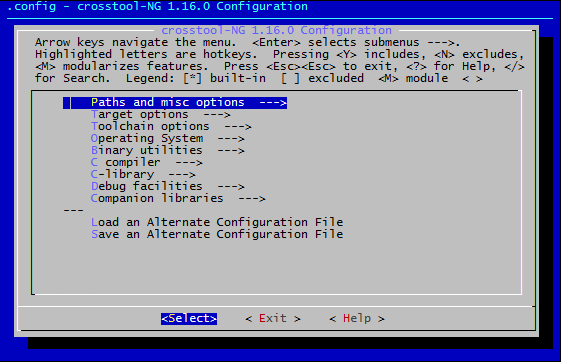
\includegraphics[scale=.5]{image/crosstool-ng.png} 
\end{center}
\end{frame}

\begin{frame}[fragile]
\frametitle{Crosstool-ng - Paths and misc options}
\begin{itemize}
\item Try features marked as EXPERIMENTAL
\item (Optional) Prefix directory: \begin{verbatim}
/opt/cross/x-tools/${CT_TARGET}
\end{verbatim}
\end{itemize}
\begin{center}
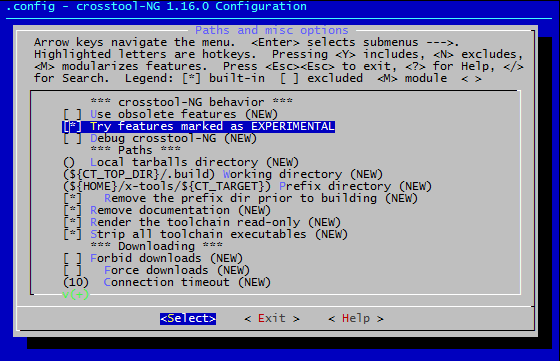
\includegraphics[scale=.4]{image/crosstool-ng-paths.png} 
\end{center}
\end{frame}

\begin{frame}
\frametitle{Crosstool-ng - Target}
\begin{itemize}
\item Target Architecture: ARM
\end{itemize}
\begin{center}
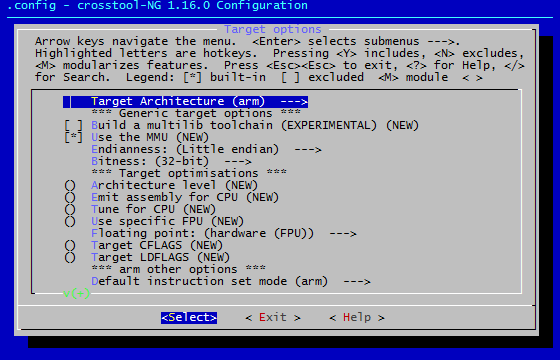
\includegraphics[scale=.4]{image/crosstool-ng-target.png} 
\end{center}
\end{frame}

\begin{frame}
\frametitle{Crosstool-ng - Operating System}
\begin{itemize}
\item Target OS: linux
\end{itemize}
\begin{center}
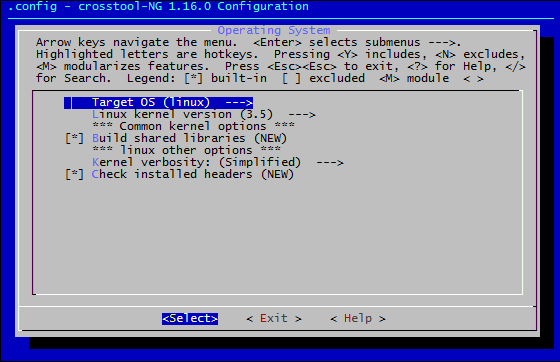
\includegraphics[scale=.4]{image/crosstool-ng-os.png} 
\end{center}
\end{frame}

\begin{frame}
\frametitle{Crosstool-ng - C compiler}
\begin{small}
\begin{itemize}
\item Show Linaro versions
\item gcc version: linaro-4.6-2012.07 (EXPERIMENTAL)
\item C++
\end{itemize}
\end{small}
\begin{center}
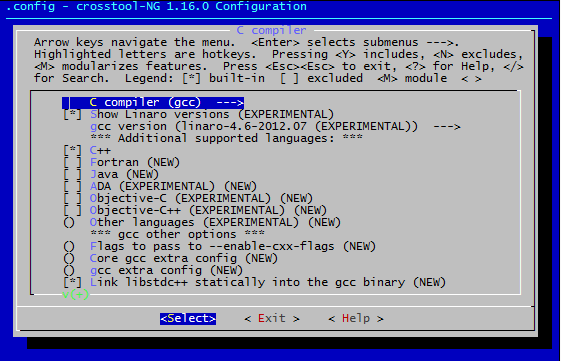
\includegraphics[scale=.4]{image/crosstool-ng-c-compiler.png} 
\end{center}
\end{frame}

\begin{frame}
\frametitle{Crosstool-ng - C-library}
\begin{small}
\begin{itemize}
\item C library: glibc
\item glibc version: 2.13
\end{itemize}
\end{small}
\begin{center}
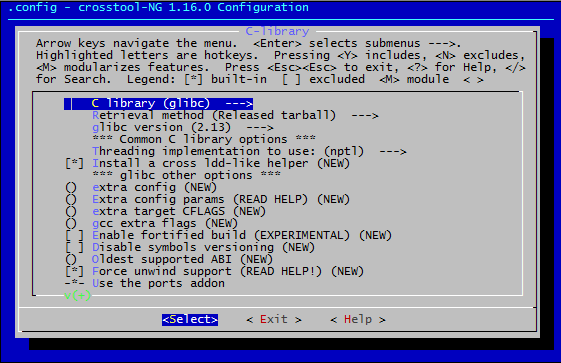
\includegraphics[scale=.4]{image/crosstool-ng-c-library.png} 
\end{center}
\end{frame}

\begin{frame}[fragile]
\frametitle{Crosstool-ng - build}
\begin{itemize}
\item Exit und Speichern
\item \begin{verbatim}
/opt/cross/bin/ct-ng build
\end{verbatim}
\item Warten ...
\end{itemize}
\begin{center}

\includegraphics[scale=.15]{image/Kaffeetasse.jpg} 
\end{center}
\end{frame}

\section{TrueCrypt}

\begin{frame}
\begin{center}
\begin{Huge}
TrueCrypt
\end{Huge}
\end{center}
\end{frame}

\begin{frame}[fragile]
\frametitle{Vorbereitung}
\begin{itemize}
\item Download und (ggf.) entpacken von:
\begin{itemize}
\item TrueCrypt-Sourcode von http://www.truecrypt.org/downloads2
\item pkcs11.h, pkcs11f.h, pkcs11t.h von ftp://ftp.rsasecurity.com/pub/pkcs/pkcs-11/v2-20/
\item wxWidgets 2.8 von http://www.wxwidgets.org
\item libfuse.a von !!!BITTE EINFÜGEN!!! (kann alternativ auch vom Raspberry Pi kopiert werden)
\end{itemize}
\item libfuse.a verschieben nach
\begin{footnotesize}
\begin{verbatim}
/opt/cross/x-tools/arm-unknown-linux-gnueabi/
arm-unknown-linux-gnueabi/sysroot/usr/lib
\end{verbatim}
\end{footnotesize}
\item Wechseln in Ordner des entpackten TrueCrypt-Source
\item Hinzufügen der Toolchain zum Path: 
\begin{footnotesize}
\begin{verbatim}
PATH=$PATH:/opt/cross/x-tools/arm-unknown-linux-gnueabi/bin/
\end{verbatim}
\end{footnotesize}
\end{itemize}
\end{frame}

\begin{frame}[fragile]
\frametitle{Build Prozess - wxWidgets}
\begin{itemize}
\item wxWidgets Make-Befehl
\begin{tiny}
\begin{verbatim}
make CC=arm-unknown-linux-gnueabi-gcc CXX=arm-unknown-linux-gnueabi-g++
AR=arm-unknown-linux-gnueabi-ar AS=arm-unknown-linux-gnueabi-as
RANLIB=arm-unknown-linux-gnueabi-ranlib WX_ROOT=../wxWidgets-2.8.12/
WX_CONFIGURE_FLAGS="--host=arm-linux-gnueabihf
--enable-unicode -disable-shared --disable-dependency-tracking --disable-compat26
--enable-exceptions --enable-std_string --enable-dataobj --enable-mimetype
--disable-protocol --disable-protocols --disable-url --disable-ipc --disable-sockets
--disable-fs_inet --disable-ole --disable-docview --disable-clipboard --disable-help
--disable-html --disable-mshtmlhelp --disable-htmlhelp --disable-mdi --disable-metafile
--disable-webkit --disable-xrc --disable-aui --disable-postscript --disable-printarch
--disable-arcstream --disable-fs_archive --disable-fs_zip --disable-tarstream
--disable-zipstream --disable-animatectrl --disable-bmpcombobox --disable-calendar
--disable-caret --disable-checklst --disable-collpane --disable-colourpicker
--disable-comboctrl --disable-datepick --disable-display --disable-dirpicker
--disable-filepicker --disable-fontpicker --disable-grid  --disable-dataviewctrl
--disable-listbook --disable-odcombobox --disable-sash  --disable-searchctrl
--disable-slider --disable-splitter --disable-togglebtn --disable-toolbar
--disable-tbarnative --disable-treebook --disable-toolbook --disable-tipwindow
--disable-popupwin --disable-commondlg --disable-aboutdlg --disable-coldlg --disable-finddlg
--disable-fontdlg --disable-numberdlg --disable-splash --disable-tipdlg --disable-progressdlg
--disable-wizarddlg --disable-miniframe --disable-tooltips --disable-splines
--disable-palette --disable-richtext --disable-dialupman --disable-debugreport
--disable-filesystem --disable-graphics_ctx --disable-sound --disable-mediactrl
--disable-joystick --disable-apple_ieee --disable-gif --disable-pcx --disable-tga
--disable-iff --disable-gif --disable-pnm --without-expat --without-libtiff --without-libjpeg
--without-libpng -without-regex --without-zlib --disable-gui"
WXSTATIC=1 NOGUI=1 wxbuild
\end{verbatim}
\end{tiny}
\end{itemize}
\end{frame}

\begin{frame}[fragile]
\frametitle{Build Prozess - wxWidgets}
\begin{itemize}
\item wxWidgets Make-Befehl
\begin{tiny}
\begin{verbatim}
make CC=arm-unknown-linux-gnueabi-gcc CXX=arm-unknown-linux-gnueabi-g++
AR=arm-unknown-linux-gnueabi-ar AS=arm-unknown-linux-gnueabi-as
RANLIB=arm-unknown-linux-gnueabi-ranlib WX_ROOT=../wxWidgets-2.8.12/
\end{verbatim}
\color{gray}
\begin{verbatim}
WX_CONFIGURE_FLAGS="--host=arm-linux-gnueabihf
--enable-unicode -disable-shared --disable-dependency-tracking --disable-compat26
--enable-exceptions --enable-std_string --enable-dataobj --enable-mimetype
--disable-protocol --disable-protocols --disable-url --disable-ipc --disable-sockets
--disable-fs_inet --disable-ole --disable-docview --disable-clipboard --disable-help
--disable-html --disable-mshtmlhelp --disable-htmlhelp --disable-mdi --disable-metafile
--disable-webkit --disable-xrc --disable-aui --disable-postscript --disable-printarch
--disable-arcstream --disable-fs_archive --disable-fs_zip --disable-tarstream
--disable-zipstream --disable-animatectrl --disable-bmpcombobox --disable-calendar
--disable-caret --disable-checklst --disable-collpane --disable-colourpicker
--disable-comboctrl --disable-datepick --disable-display --disable-dirpicker
--disable-filepicker --disable-fontpicker --disable-grid  --disable-dataviewctrl
--disable-listbook --disable-odcombobox --disable-sash  --disable-searchctrl
--disable-slider --disable-splitter --disable-togglebtn --disable-toolbar
--disable-tbarnative --disable-treebook --disable-toolbook --disable-tipwindow
--disable-popupwin --disable-commondlg --disable-aboutdlg --disable-coldlg --disable-finddlg
--disable-fontdlg --disable-numberdlg --disable-splash --disable-tipdlg --disable-progressdlg
--disable-wizarddlg --disable-miniframe --disable-tooltips --disable-splines
--disable-palette --disable-richtext --disable-dialupman --disable-debugreport
--disable-filesystem --disable-graphics_ctx --disable-sound --disable-mediactrl
--disable-joystick --disable-apple_ieee --disable-gif --disable-pcx --disable-tga
--disable-iff --disable-gif --disable-pnm --without-expat --without-libtiff --without-libjpeg
--without-libpng -without-regex --without-zlib --disable-gui"
WXSTATIC=1 NOGUI=1 wxbuild
\end{verbatim}
\end{tiny}
\end{itemize}
\end{frame}

\begin{frame}[fragile]
\frametitle{Build Prozess - wxWidgets}
\begin{itemize}
\item wxWidgets Make-Befehl
\begin{tiny}
\color{gray}
\begin{verbatim}
make CC=arm-unknown-linux-gnueabi-gcc CXX=arm-unknown-linux-gnueabi-g++
AR=arm-unknown-linux-gnueabi-ar AS=arm-unknown-linux-gnueabi-as
RANLIB=arm-unknown-linux-gnueabi-ranlib WX_ROOT=../wxWidgets-2.8.12/
\end{verbatim}
\color{black}
\begin{verbatim}
WX_CONFIGURE_FLAGS="--host=arm-linux-gnueabihf
--enable-unicode -disable-shared --disable-dependency-tracking --disable-compat26
--enable-exceptions --enable-std_string --enable-dataobj --enable-mimetype
--disable-protocol --disable-protocols --disable-url --disable-ipc --disable-sockets
--disable-fs_inet --disable-ole --disable-docview --disable-clipboard --disable-help
--disable-html --disable-mshtmlhelp --disable-htmlhelp --disable-mdi --disable-metafile
--disable-webkit --disable-xrc --disable-aui --disable-postscript --disable-printarch
--disable-arcstream --disable-fs_archive --disable-fs_zip --disable-tarstream
--disable-zipstream --disable-animatectrl --disable-bmpcombobox --disable-calendar
--disable-caret --disable-checklst --disable-collpane --disable-colourpicker
--disable-comboctrl --disable-datepick --disable-display --disable-dirpicker
--disable-filepicker --disable-fontpicker --disable-grid  --disable-dataviewctrl
--disable-listbook --disable-odcombobox --disable-sash  --disable-searchctrl
--disable-slider --disable-splitter --disable-togglebtn --disable-toolbar
--disable-tbarnative --disable-treebook --disable-toolbook --disable-tipwindow
--disable-popupwin --disable-commondlg --disable-aboutdlg --disable-coldlg --disable-finddlg
--disable-fontdlg --disable-numberdlg --disable-splash --disable-tipdlg --disable-progressdlg
--disable-wizarddlg --disable-miniframe --disable-tooltips --disable-splines
--disable-palette --disable-richtext --disable-dialupman --disable-debugreport
--disable-filesystem --disable-graphics_ctx --disable-sound --disable-mediactrl
--disable-joystick --disable-apple_ieee --disable-gif --disable-pcx --disable-tga
--disable-iff --disable-gif --disable-pnm --without-expat --without-libtiff --without-libjpeg
--without-libpng -without-regex --without-zlib --disable-gui"
WXSTATIC=1 NOGUI=1 wxbuild
\end{verbatim}
\end{tiny}
\end{itemize}
\end{frame}


\begin{frame}[fragile]
\frametitle{Build Prozess - TrueCrypt}
\begin{itemize}
\item TrueCrypt Make-Befehl: 
\begin{tiny}
\begin{verbatim}
make CC=arm-unknown-linux-gnueabi-gcc
CXX=arm-unknown-linux-gnueabi-g++ AS=arm-unknown-linux-gnueabi-as
AR=arm-unknown-linux-gnueabi-ar RANLIB=arm-unknown-linux-gnueabi-ranlib
PKCS11_INC=../ WX_ROOT=../wxWidgets-2.8.12/ WXSTATIC=1 NOGUI=1 NOASM=1 NOTEST=1
\end{verbatim}
\end{tiny}
\item Binary unter:
\begin{verbatim}
Main/truecrypt
\end{verbatim}
\item Auf Raspberry Pi kopieren und ausfuehren
\end{itemize}
\end{frame}

\section{Sonstiges}

\begin{frame}
\frametitle{Abschließende Worte}
\begin{itemize}
\item Grundsätzlich jedes Programm das Toolchain nutzt übersetzbar
\item Makefiles müssen eigene Toolchain erlauben
\item Für statisches Linken, Bibliotheken der Zielarchitektur benötigt
\item Einblick in Makefiles manchmal sehr aufschlussreich\\
\begin{large}
\begin{center}
\textit{Use the source, Luke!}
\end{center}
\end{large}
\end{itemize}
\end{frame}

\begin{frame}
\begin{Huge}
\begin{center}
Fragen?
\end{center}
\end{Huge}
\end{frame}


\end{document}
